%-------------------------------------------------------
\section{\label{sec:back:syncasync}Synchronous and Asynchronous Messaging in Distributed Algorithms}
%-------------------------------------------------------

This dissertation uses the standard timing models in distributed algorithms \cite{Lynch1996} for messaging where relevant.  For reference, the most important relevant concepts are explained and illustrated below.  For more on the topics discussed in this \lcnamecref{sec:back:syncasync}, the interested reader is referred to \cite{Fokkink2013,Lynch1996,Tel2000}.

\subsection{Rounds}
Under both synchronous and asynchronous messaging, all processes work in \emph{rounds} (sometimes also referred to as \emph{macro-steps}).  A round consists of three repeating sequential sub-steps:
\begin{enumerate}
    \item \emph{\textsf{Receive}}:  receive one or more incoming messages
    \item \emph{\textsf{Process}}:  perform any requisite local computations, and update the local state
    \item \emph{\textsf{Send}}:  send out new messages as appropriate based on the processing from the previous step
\end{enumerate}
This applies only to messaging between processes.  For systems with a solitary process, there is no meaningful difference because the process will essentially remain in the \textsf{process} sub-step.  \Ie{} a lone process will continue working without messaging until the system halts (if ever).

\subsection{Synchronous Messaging}
Under the synchronous model, all processes proceed in lock-step.  They may carry out the sub-steps at different speeds, but begin and end rounds together.  When considering timing of messaging, there are two standard approaches:  to consider the \textsf{process} sub-step as taking one time unit and the transit time -- the time between when the message is sent by the sender and when it is received by the recipient -- taking zero time units; or, to consider the \textsf{process} sub-step as taking zero time units and the transit time taking one time unit.

\subsection{Asynchronous Messaging}
Under the asynchronous model, there is (unsurprisingly) no natural synchronisation between processes.  All processes proceed through the sub-steps at their own pace.  The \textsf{process} sub-step is considered to take zero time units, and transit times are considered to take any number of time units.  Alternatively, by normalisation, while the \textsf{process} sub-step still takes zero time units, transit times take somewhere between zero and one (inclusive) time units.  This makes the second synchronous approach a special case of the asynchronous approach.  The asynchronous model is similar to the theoretical \gls{actor} model.

\subsection{Echo}
To illustrate the difference between the synchronous and asynchronous scenarios, consider the illustrations in \cref{fig:back:echosync,fig:back:echoasync}.\footnote{These figures were created by Dr. Radu Nicolescu, and have been reproduced here with his permission.}  The \textsf{echo} algorithm \cite[Ch.~4.3]{Fokkink2013} is used to establish a spanning tree over a graph of nodes/processes, in this case rooted at node 1.  The algorithm works in two phases, named \emph{broadcast} and \emph{convergecast}.  \textsf{Echo} starts in the broadcast phase with an initiator node sending out a broadcast message to each of its neighbours.  Each of those recipients then marks the sender as its parent, and in turn sends a broadcast message to every other one of its neighbours, then waits to receive a broadcast message from each of those other neighbours.  This pattern repeats across the graph.  Once the response broadcast messages are received, each node then sends a convergecast message back to its parent.  This carries on until finally the initiator receives the convergecast messages back from its neighbours.

In \cref{fig:back:echosync,fig:back:echoasync}, the first green node is the initiator, and each other node turns green when it receives its first message.  Edges between nodes turn into green arrows when a node chooses its parent.  The direction of the arrow points to said parent.  Red arrows indicate the direction of travel for a broadcast message, while blue arrows indicate the direction of travel for a convergecast message.  Solid red \& blue arrows indicate that a message is received in that round by the recipient, while a dashed line indicates that the message is still in transit.

\begin{figure}[htbp]
    \centering
    \subcaptionbox{Round Zero}{\includegraphics[width=0.32\textwidth]{chapters/background/images/echo/sync/notext_f0_0.pdf}}
    \subcaptionbox{Round One}{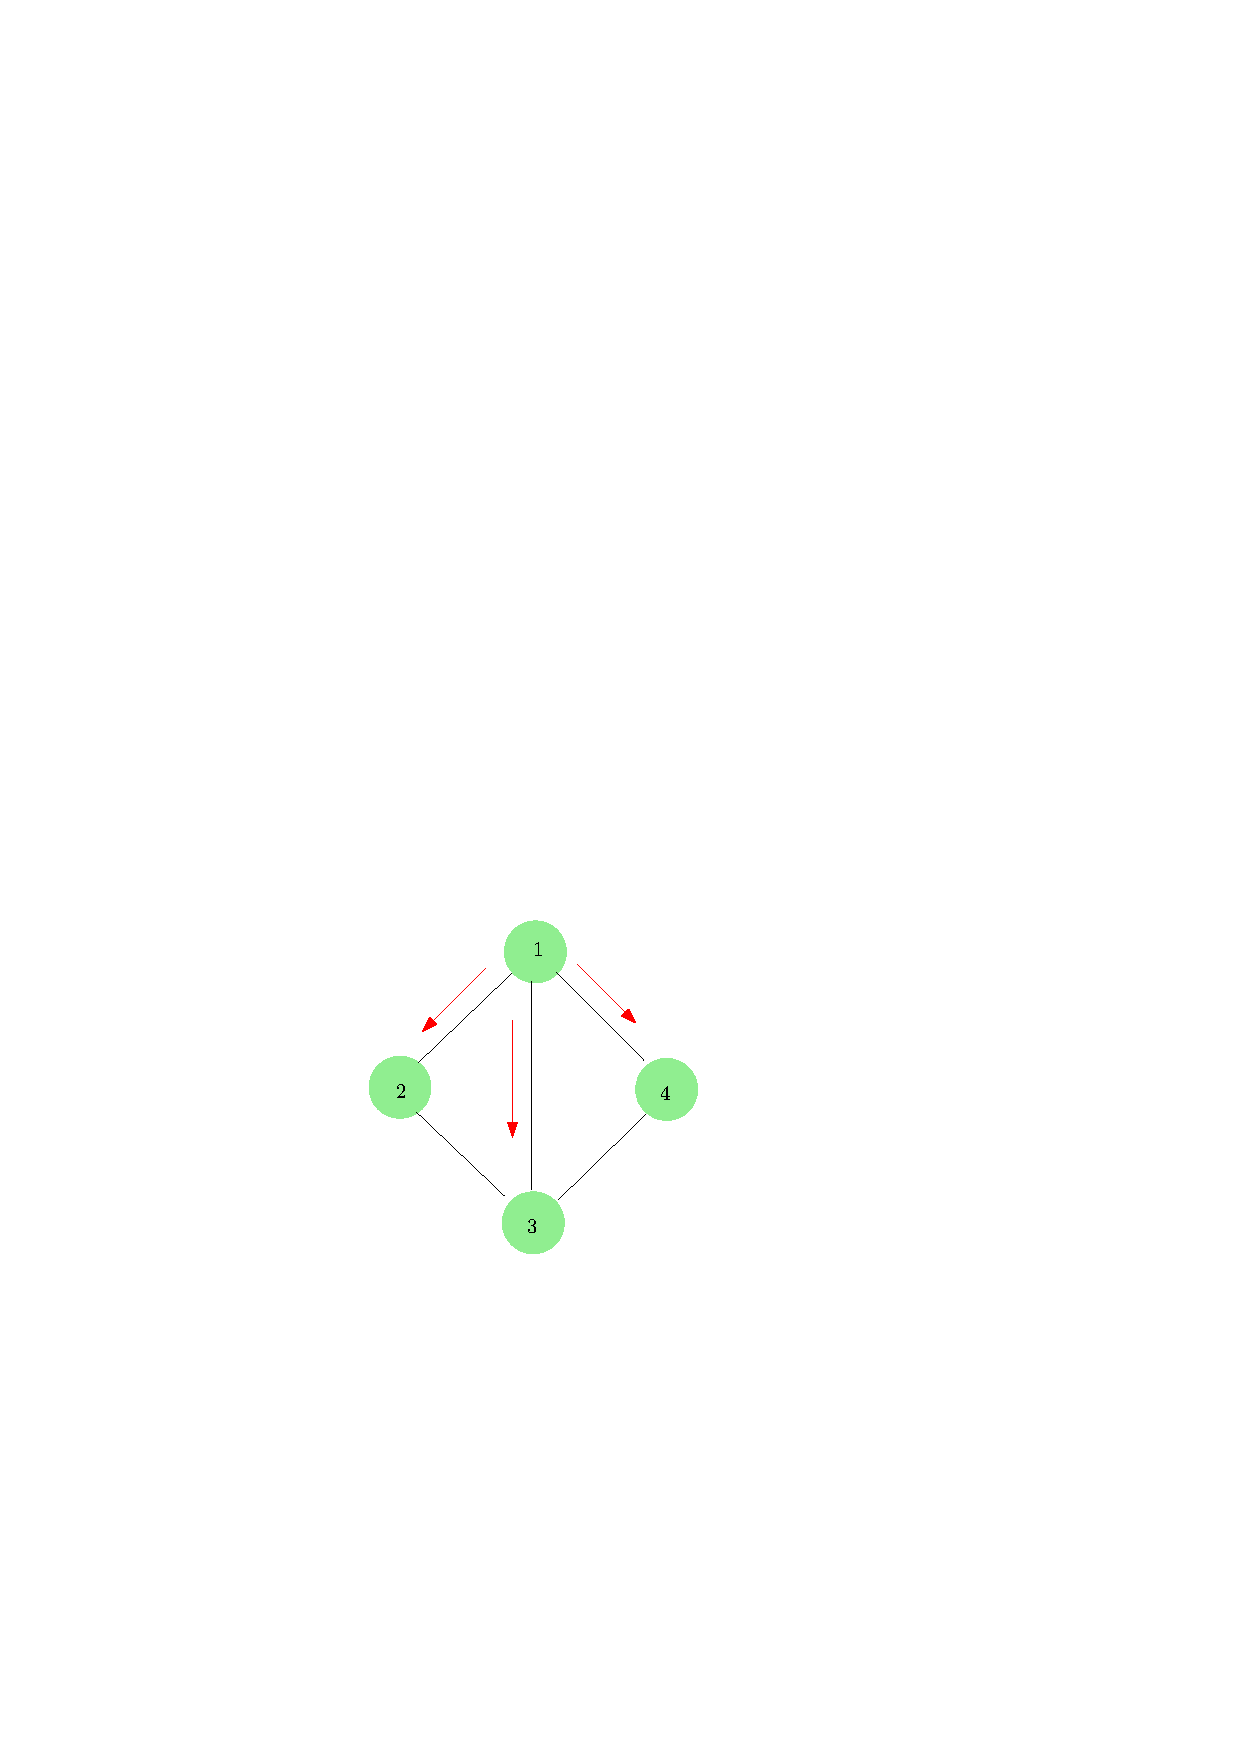
\includegraphics[width=0.32\textwidth]{chapters/background/images/echo/sync/notext_f0_1.pdf}}
    \subcaptionbox{Round Two}{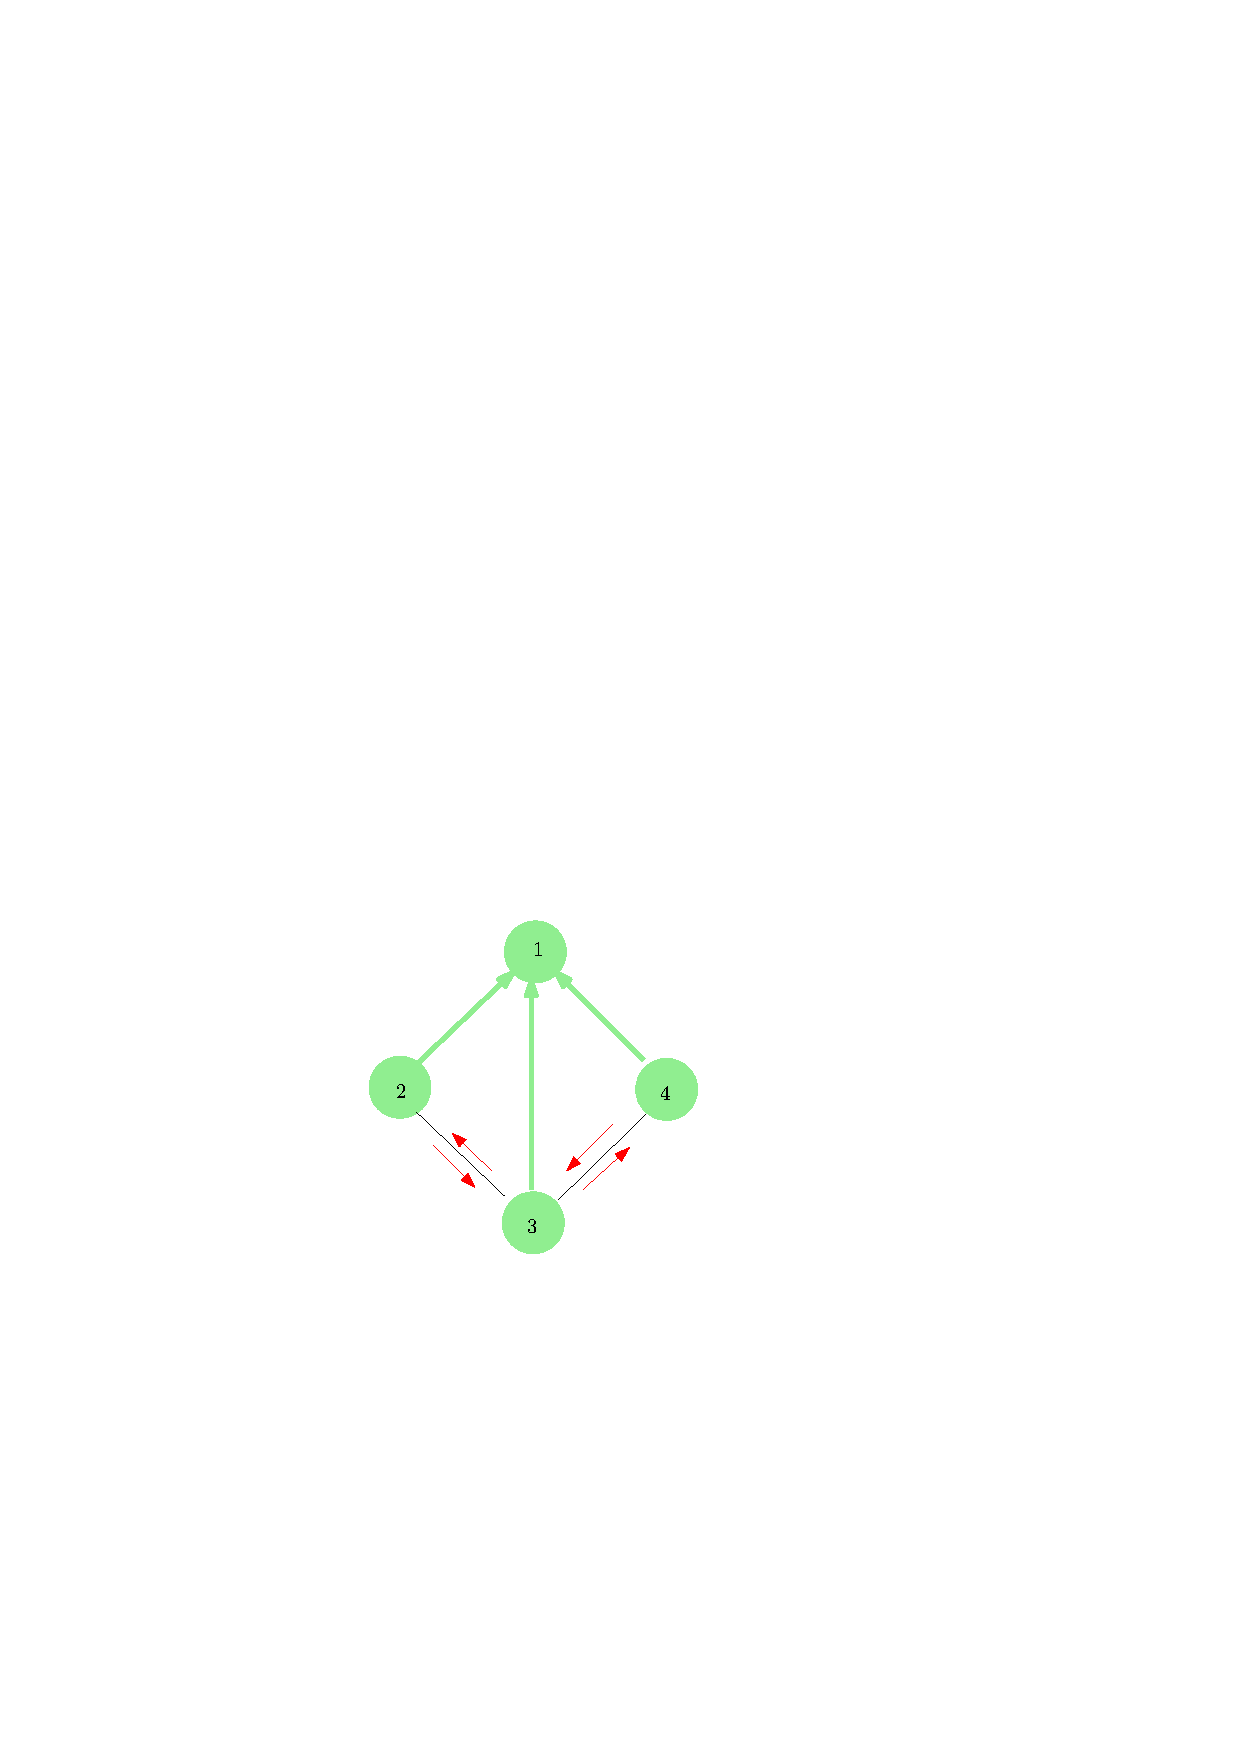
\includegraphics[width=0.32\textwidth]{chapters/background/images/echo/sync/notext_f0_2.pdf}}
    \subcaptionbox{Round Three}{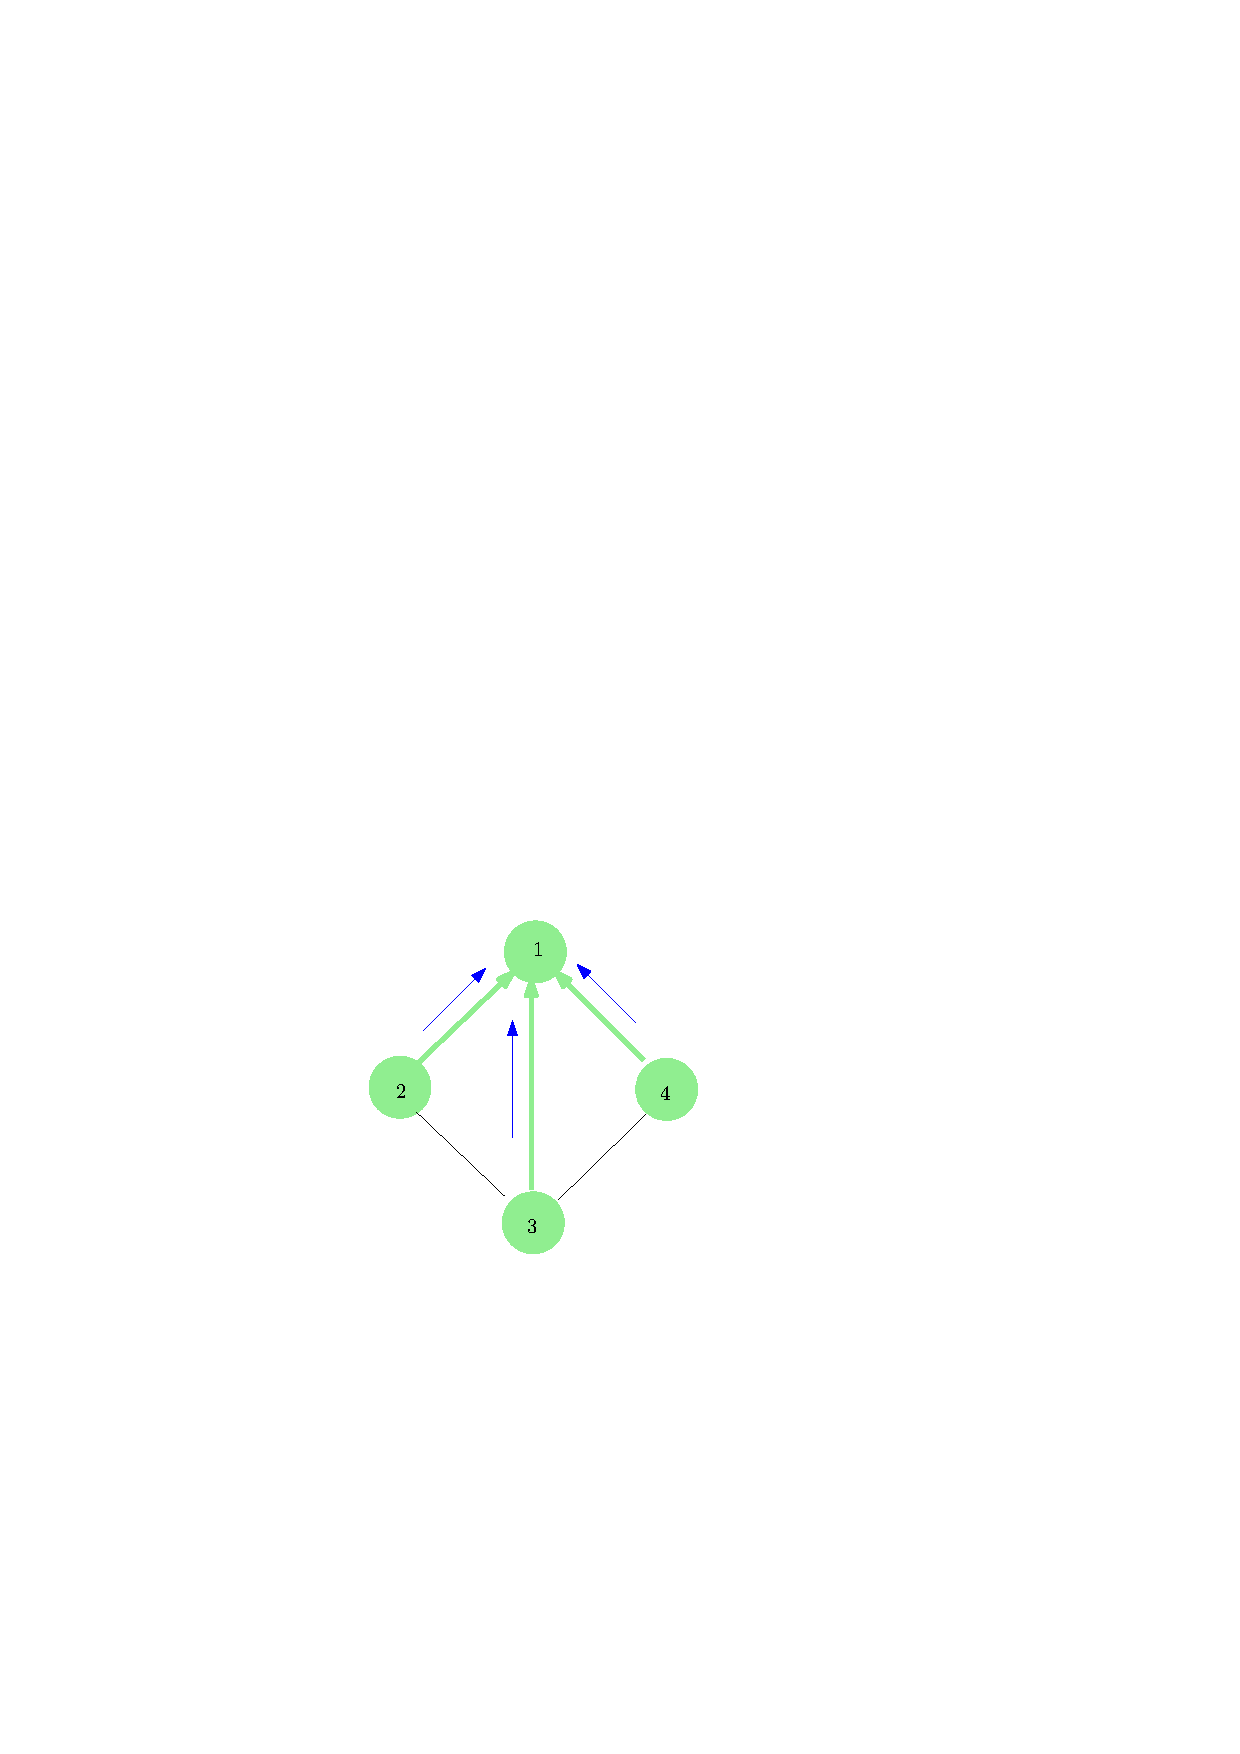
\includegraphics[width=0.32\textwidth]{chapters/background/images/echo/sync/notext_f0_3.pdf}}
    \caption[Progression of the synchronous \textsf{echo} algorithm]{Progression of the synchronous \textsf{echo} algorithm, starting from round zero before any messages are sent.  Arrows in red mean broadcast messages, while arrows in blue mean convergecast messages.}
    \label{fig:back:echosync}
\end{figure}

\begin{figure}[htbp]
    \centering
    \subcaptionbox{Round Zero}{\includegraphics[width=0.32\textwidth]{chapters/background/images/echo/async/notext_f0_0.pdf}}
    \subcaptionbox{Round One}{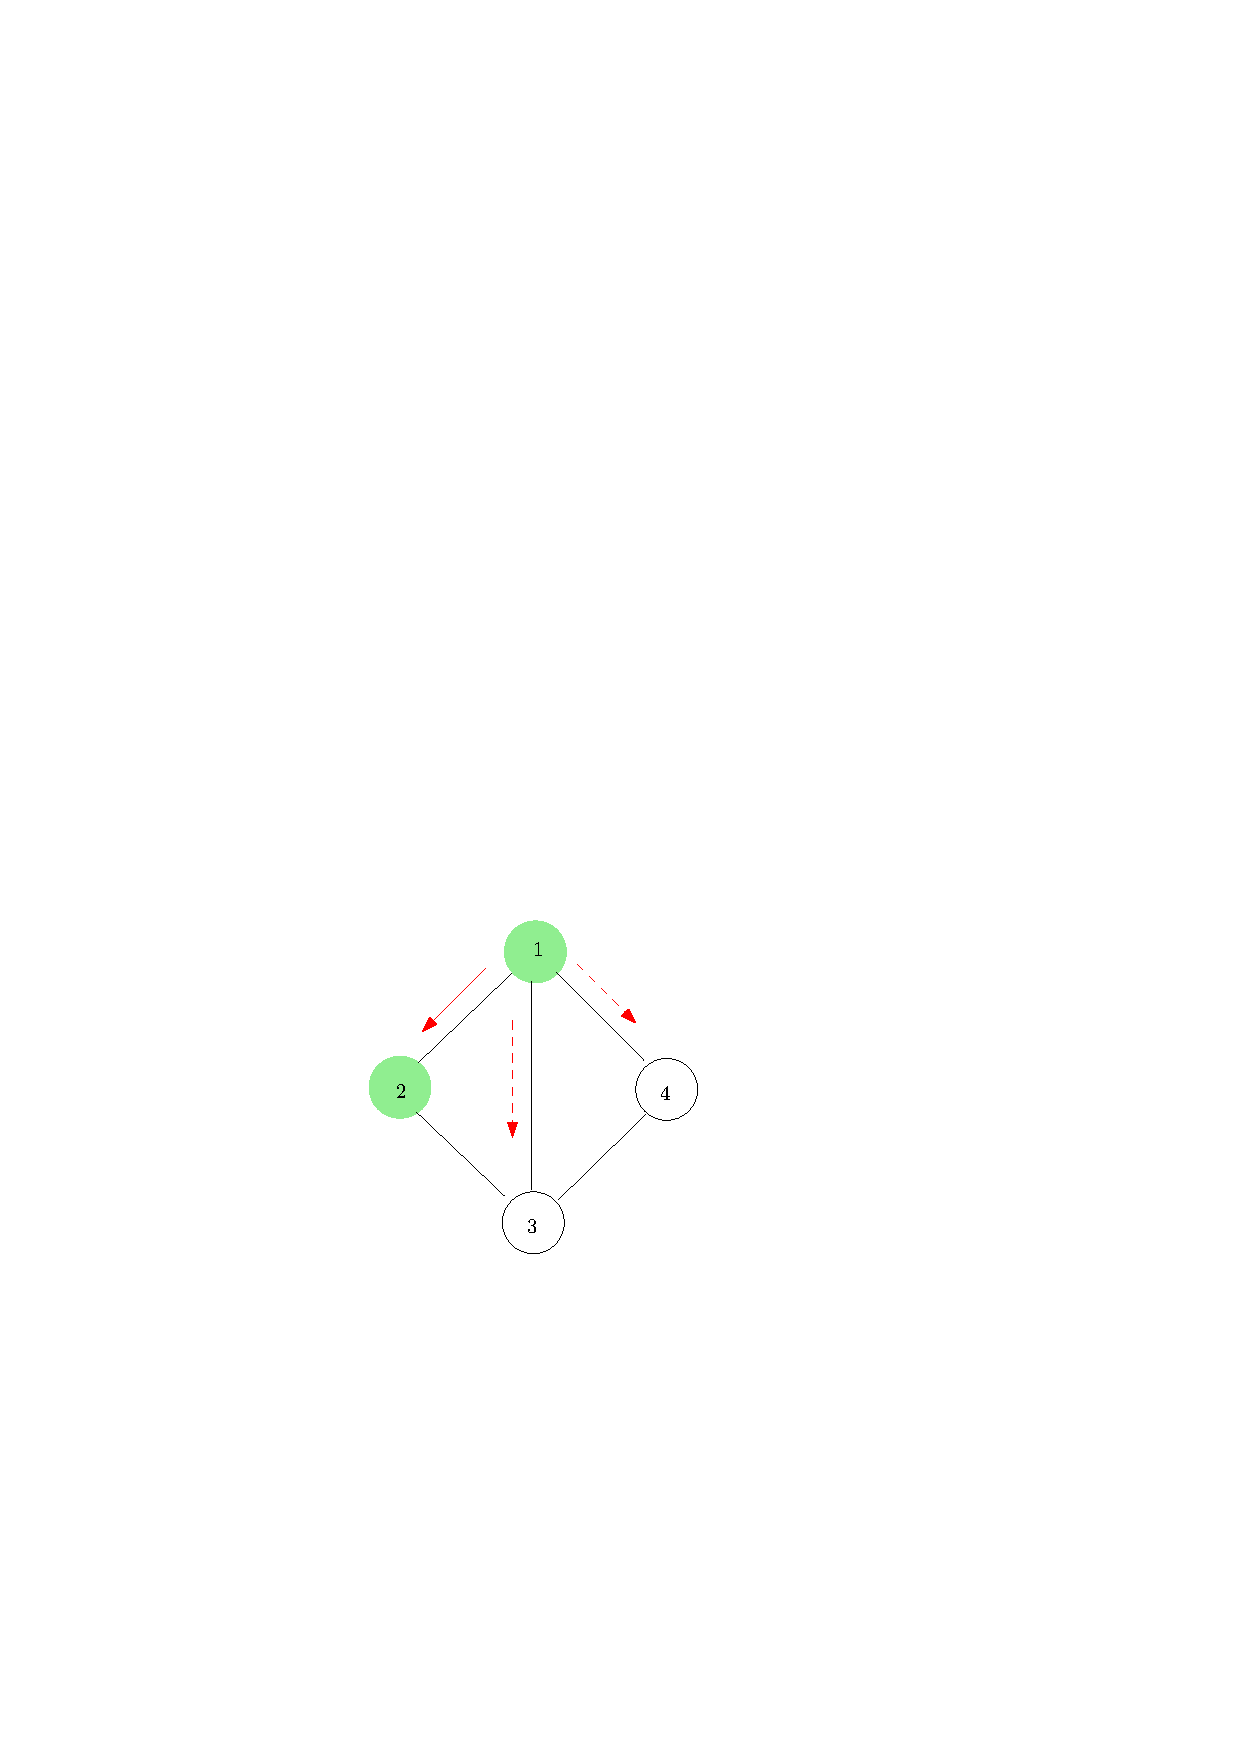
\includegraphics[width=0.32\textwidth]{chapters/background/images/echo/async/notext_f0_1.pdf}}
    \subcaptionbox{Round Two}{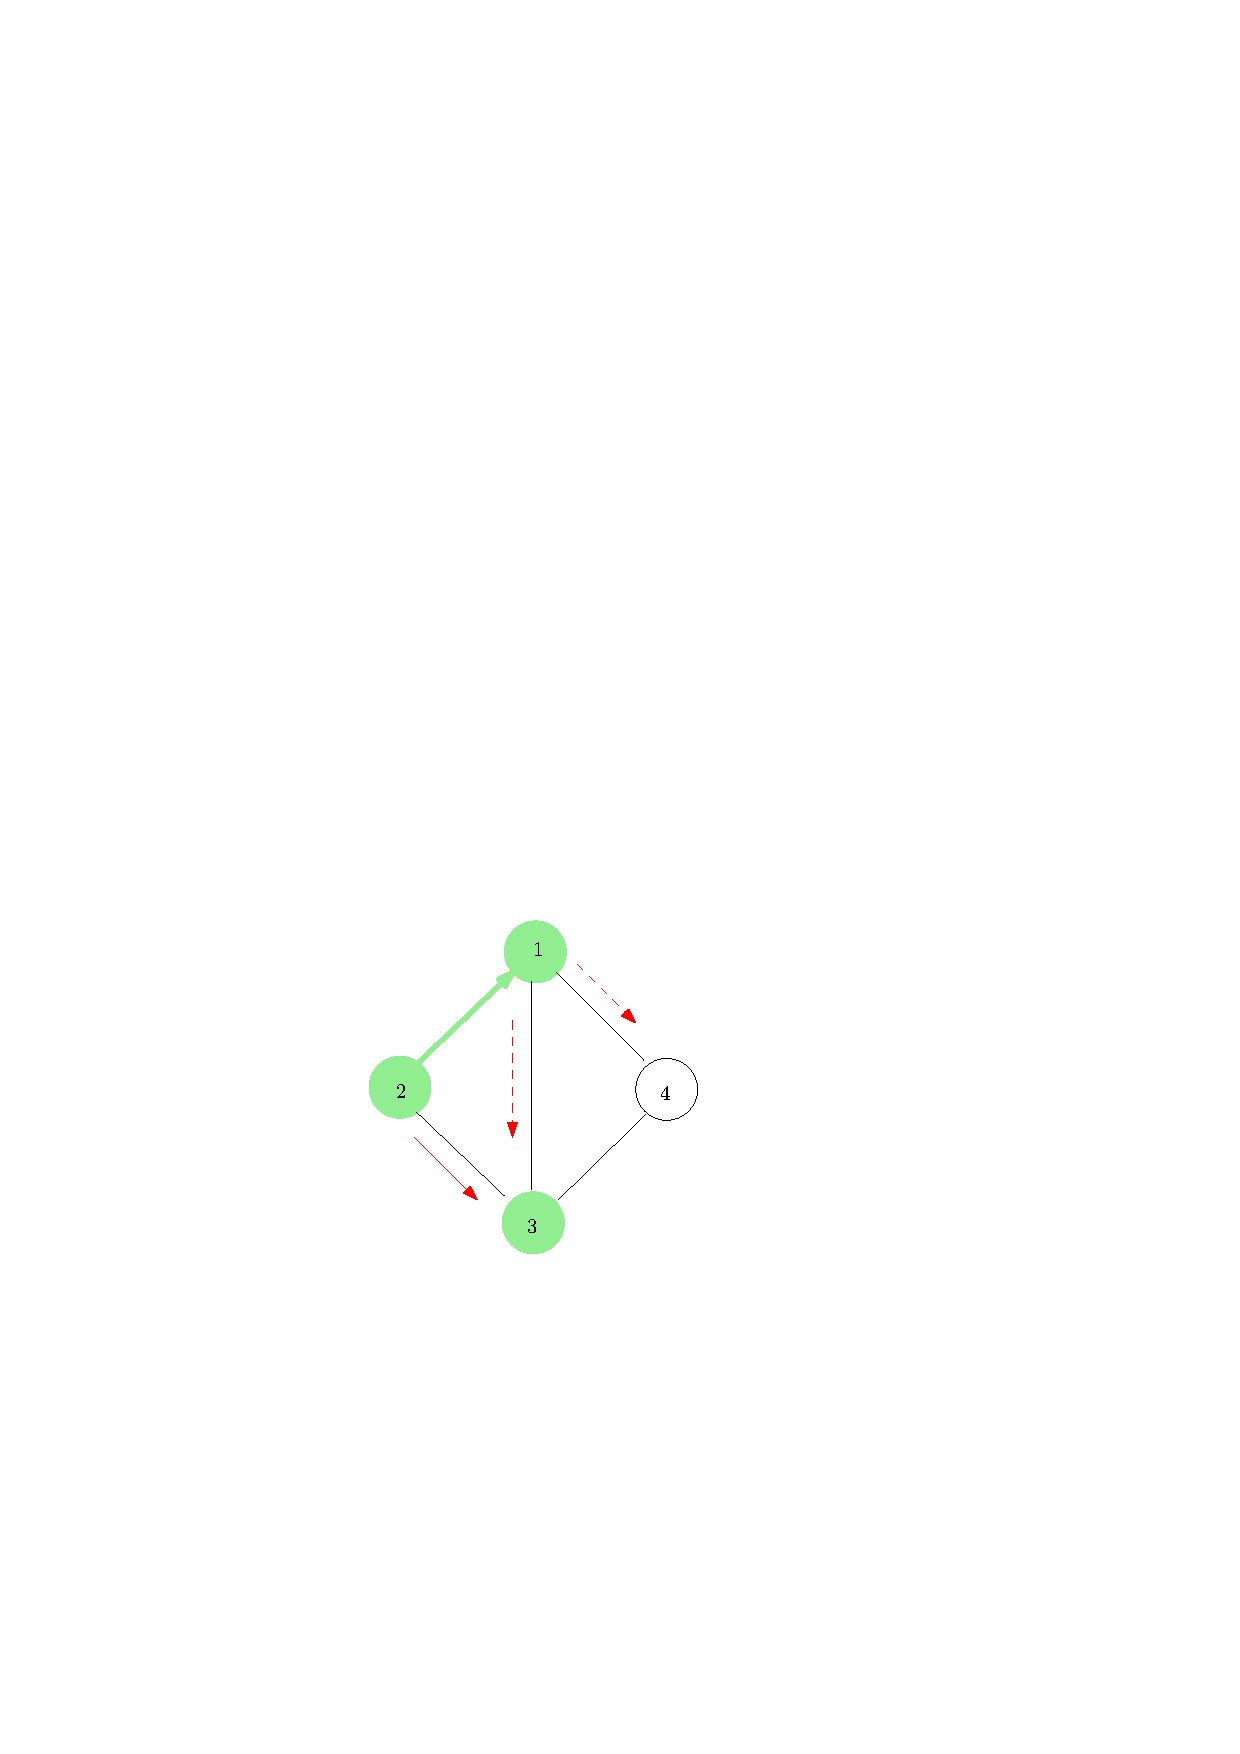
\includegraphics[width=0.32\textwidth]{chapters/background/images/echo/async/notext_f0_2.pdf}}
    \subcaptionbox{Round Three\label{fig:back:echoasync:3}}{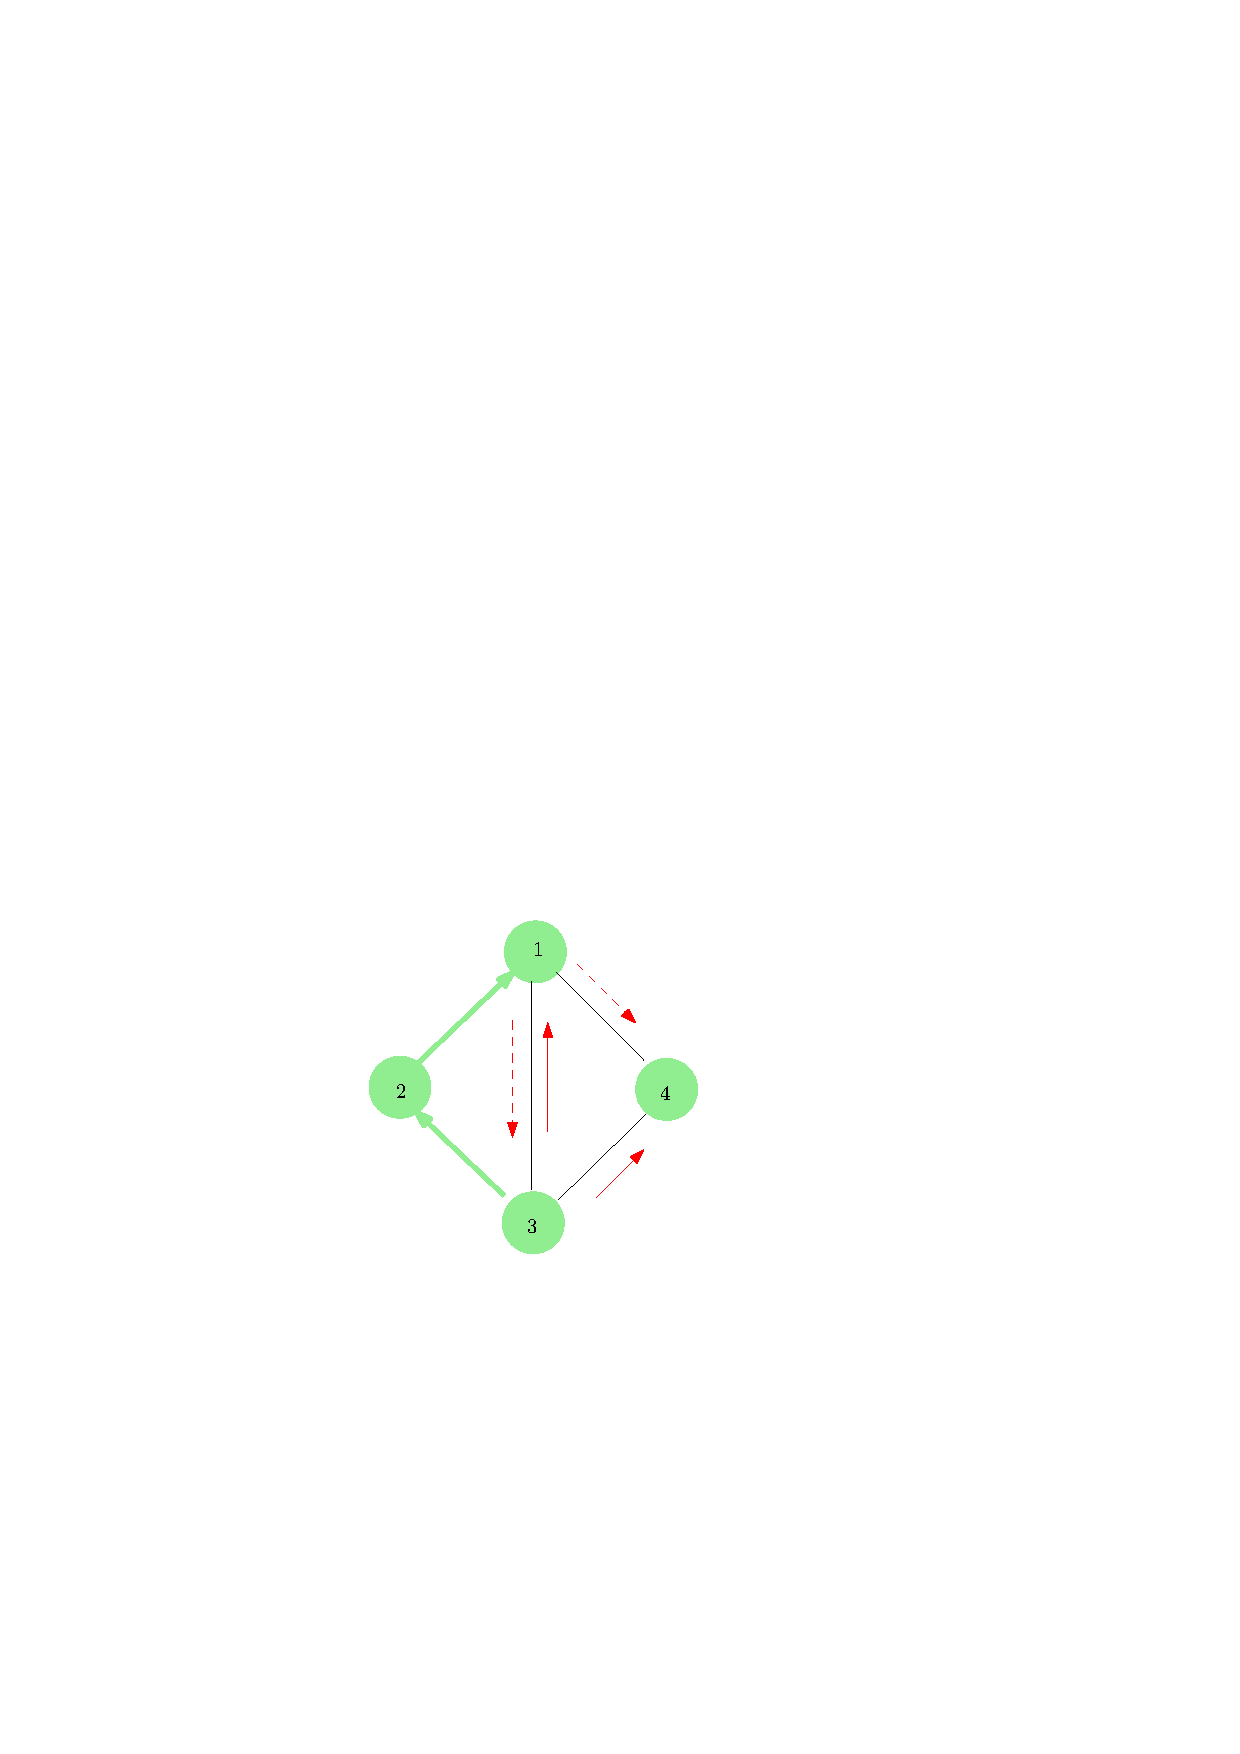
\includegraphics[width=0.32\textwidth]{chapters/background/images/echo/async/notext_f0_3.pdf}}
    \subcaptionbox{Round Four}{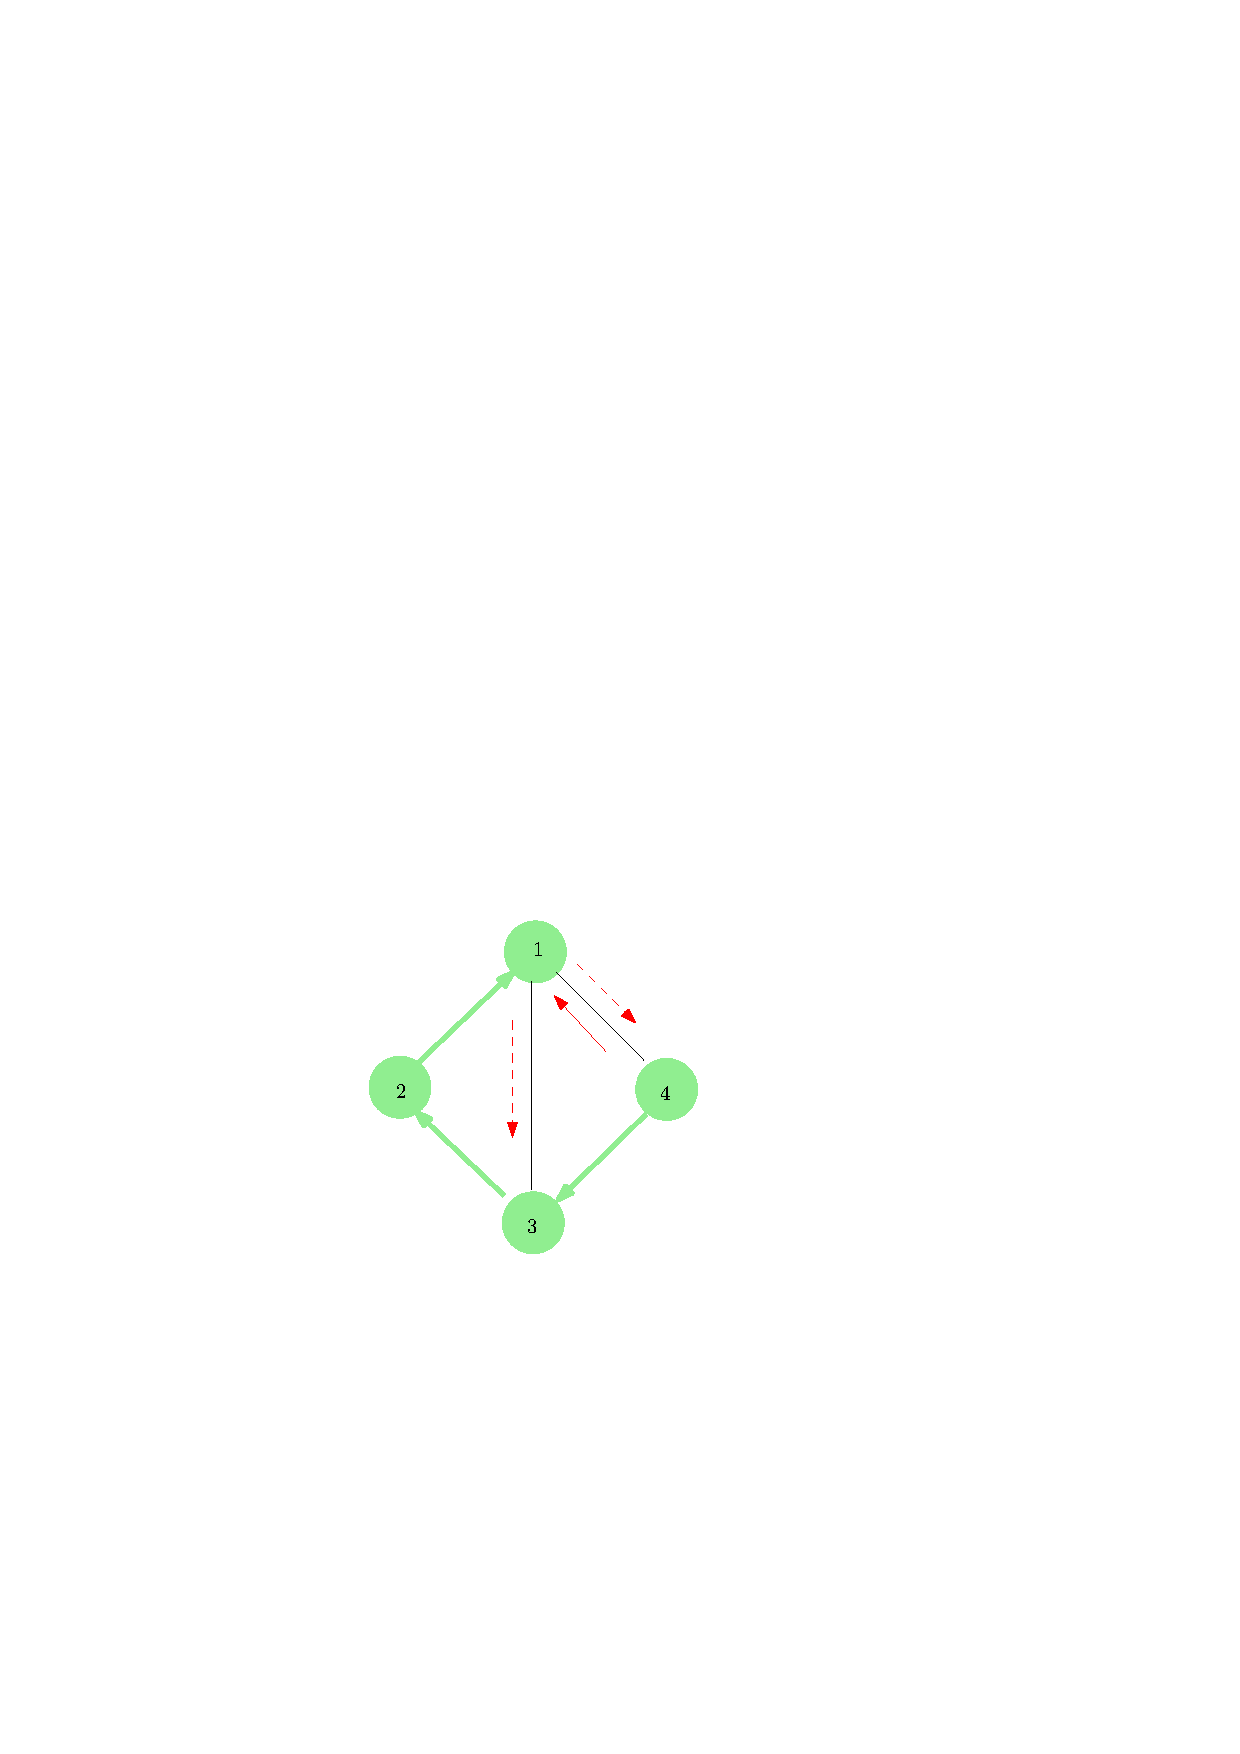
\includegraphics[width=0.32\textwidth]{chapters/background/images/echo/async/notext_f0_4.pdf}}
    \subcaptionbox{Round Five}{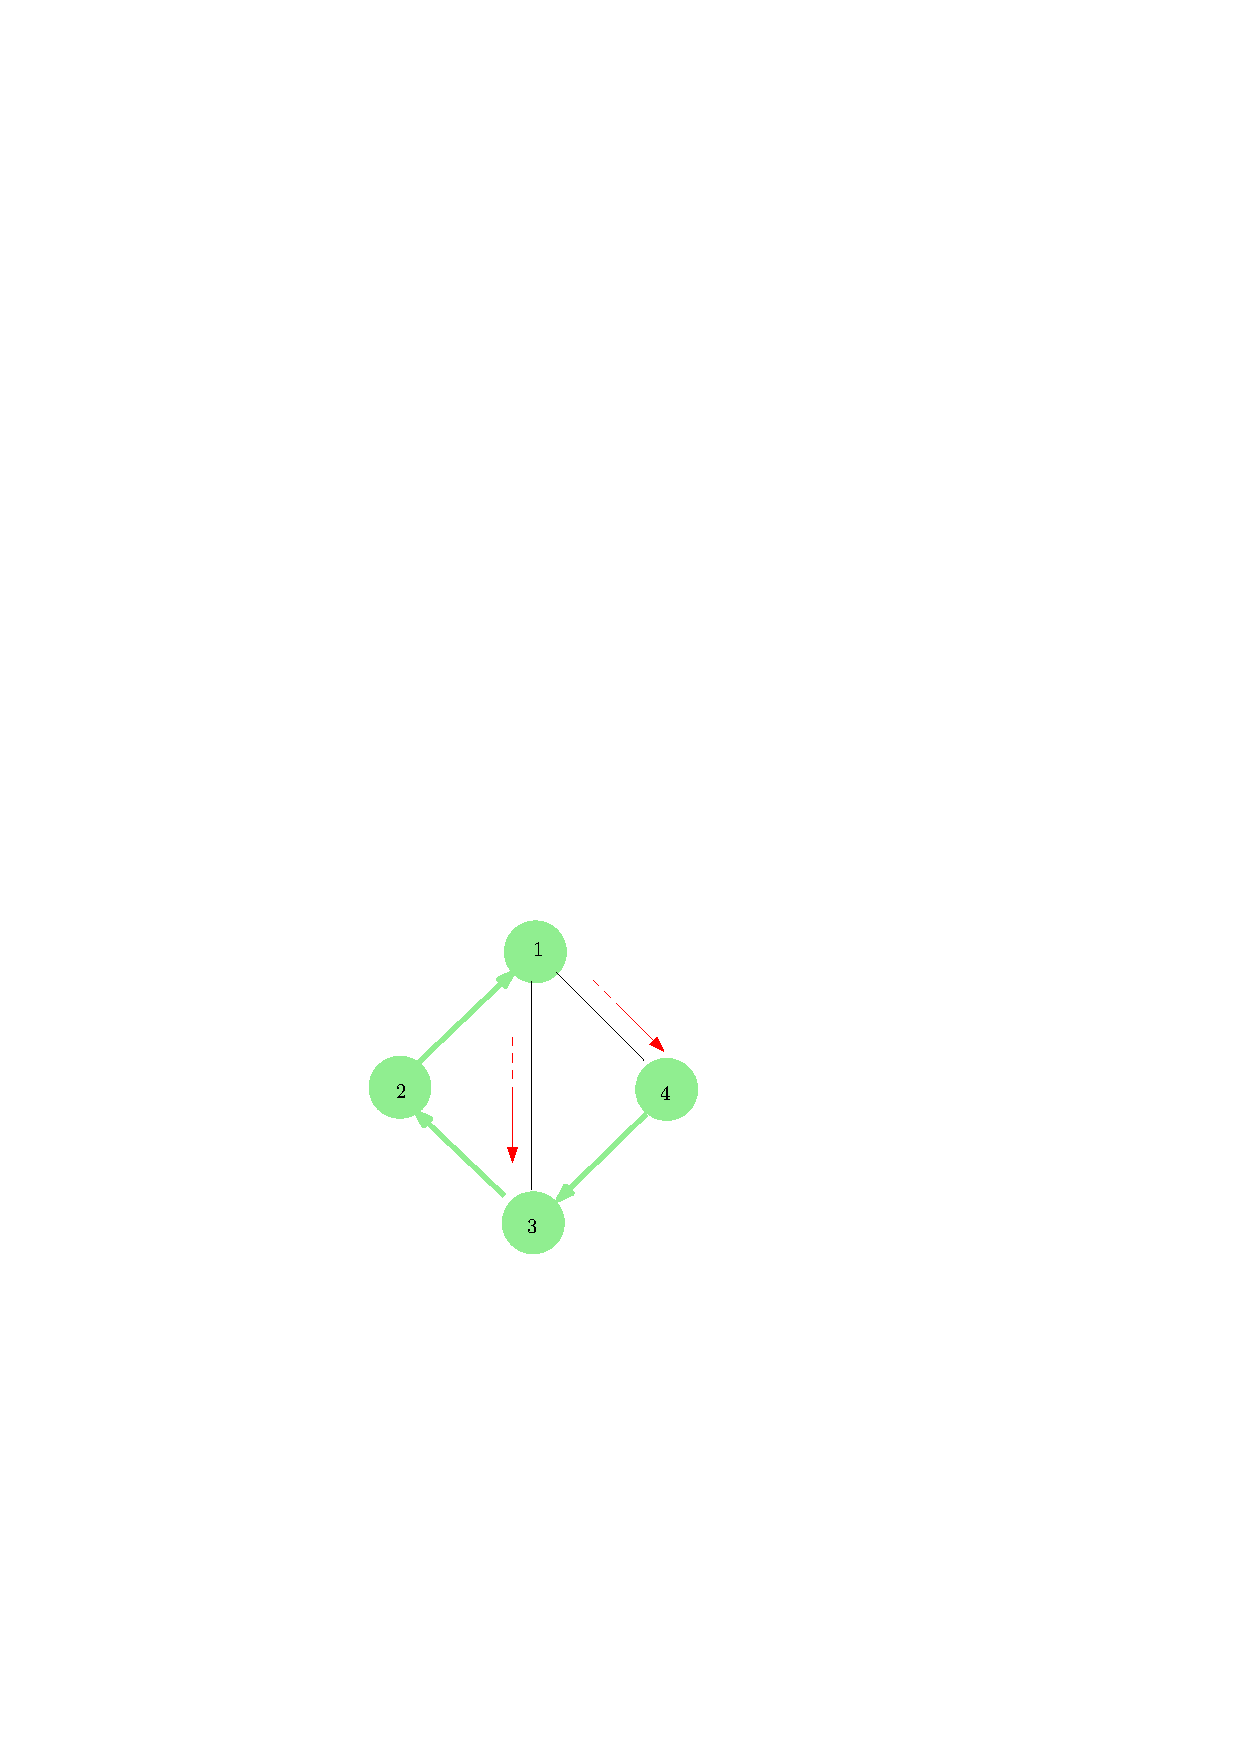
\includegraphics[width=0.32\textwidth]{chapters/background/images/echo/async/notext_f0_5.pdf}}
    \subcaptionbox{Round Six}{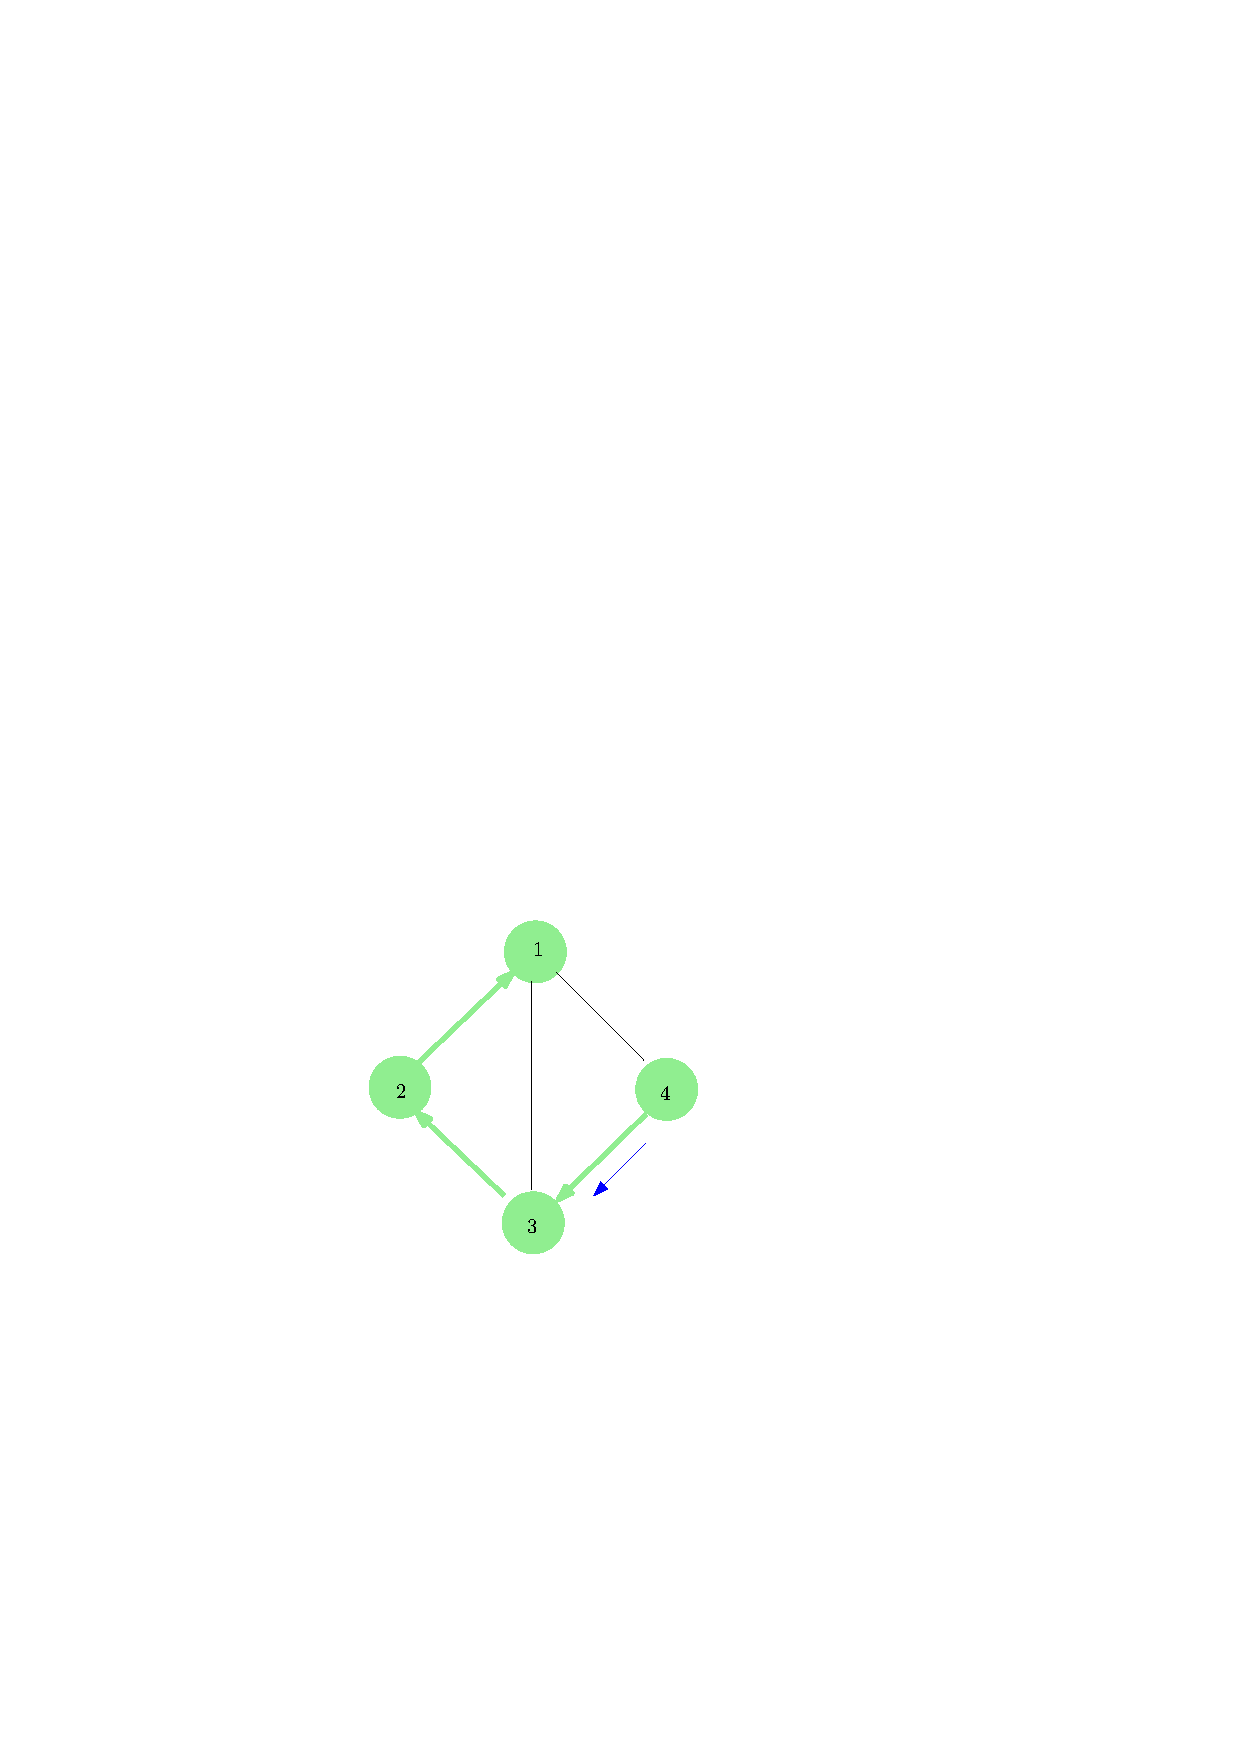
\includegraphics[width=0.32\textwidth]{chapters/background/images/echo/async/notext_f0_6.pdf}}
    \subcaptionbox{Round Seven}{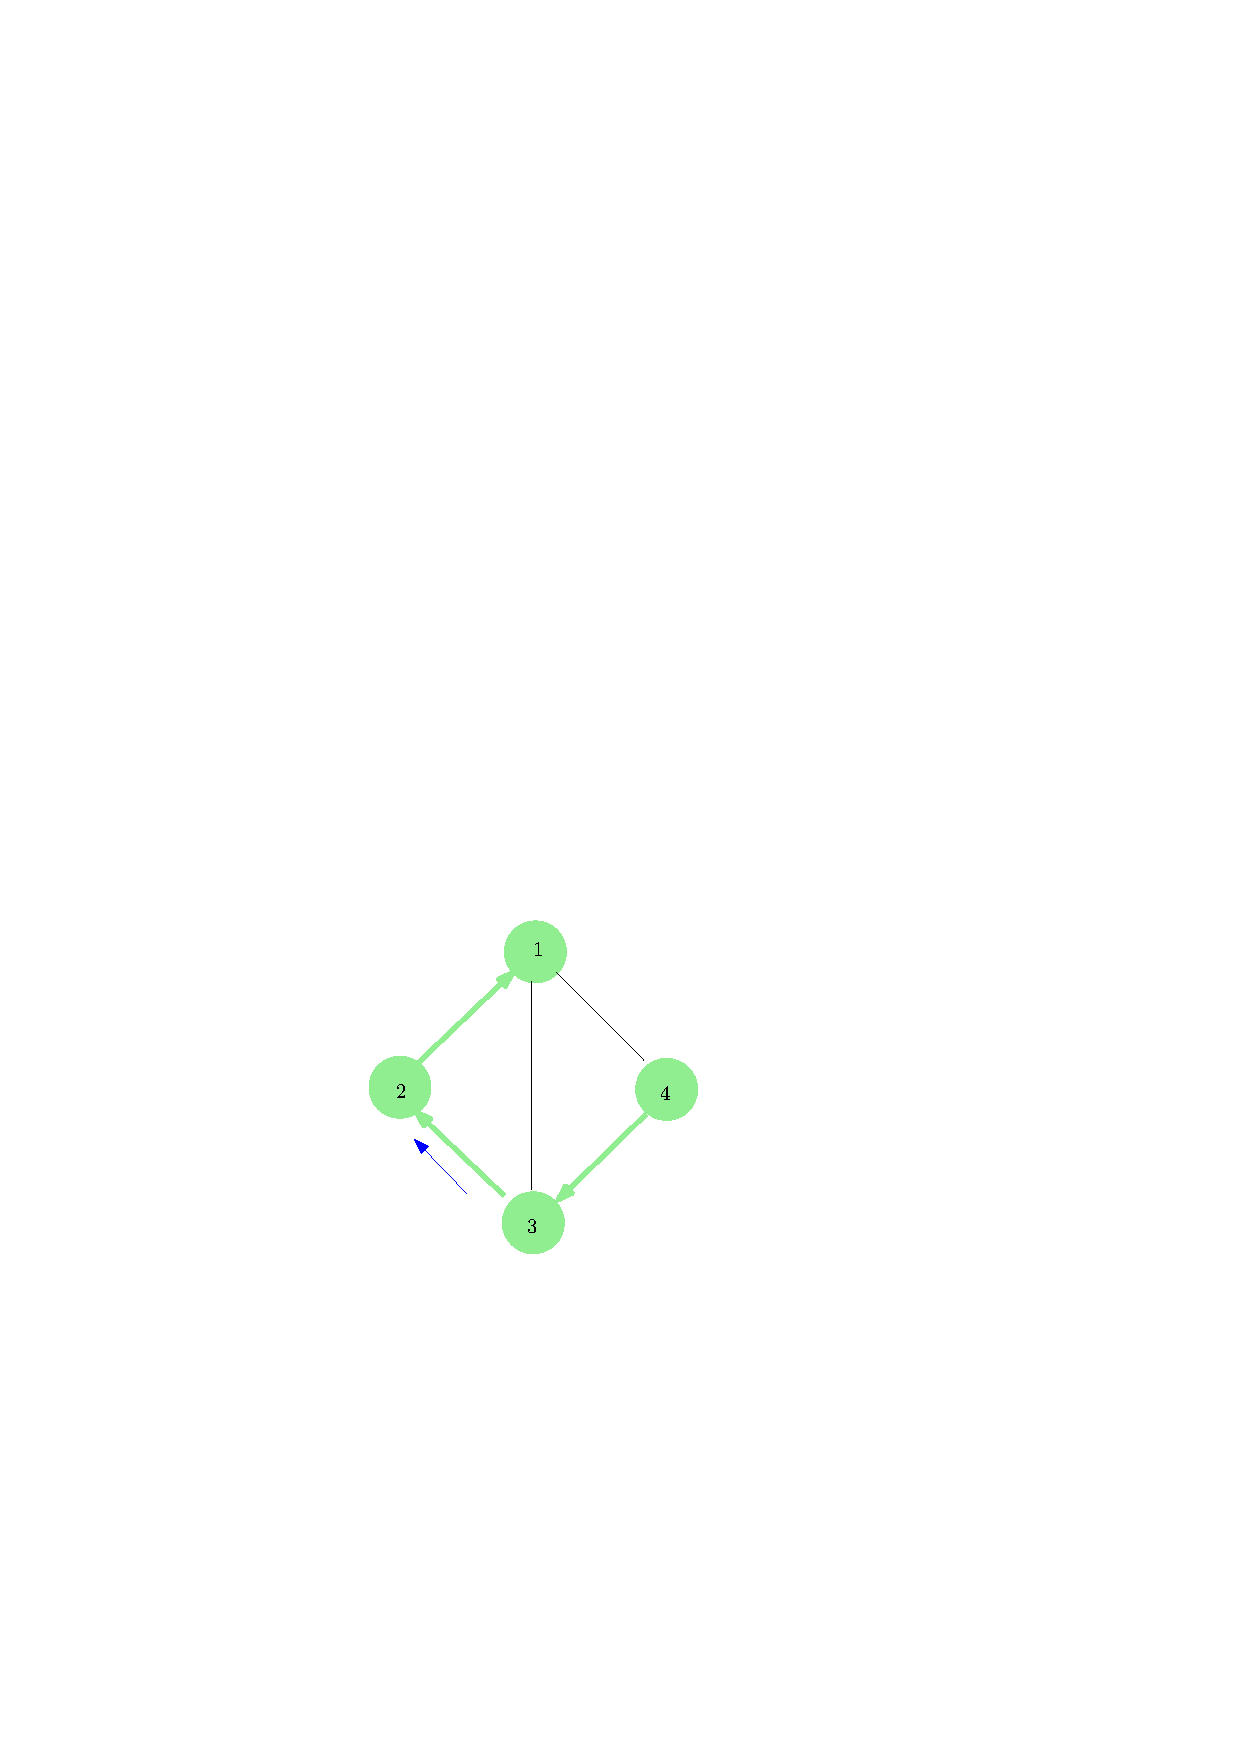
\includegraphics[width=0.32\textwidth]{chapters/background/images/echo/async/notext_f0_7.pdf}}
    \subcaptionbox{Round Eight}{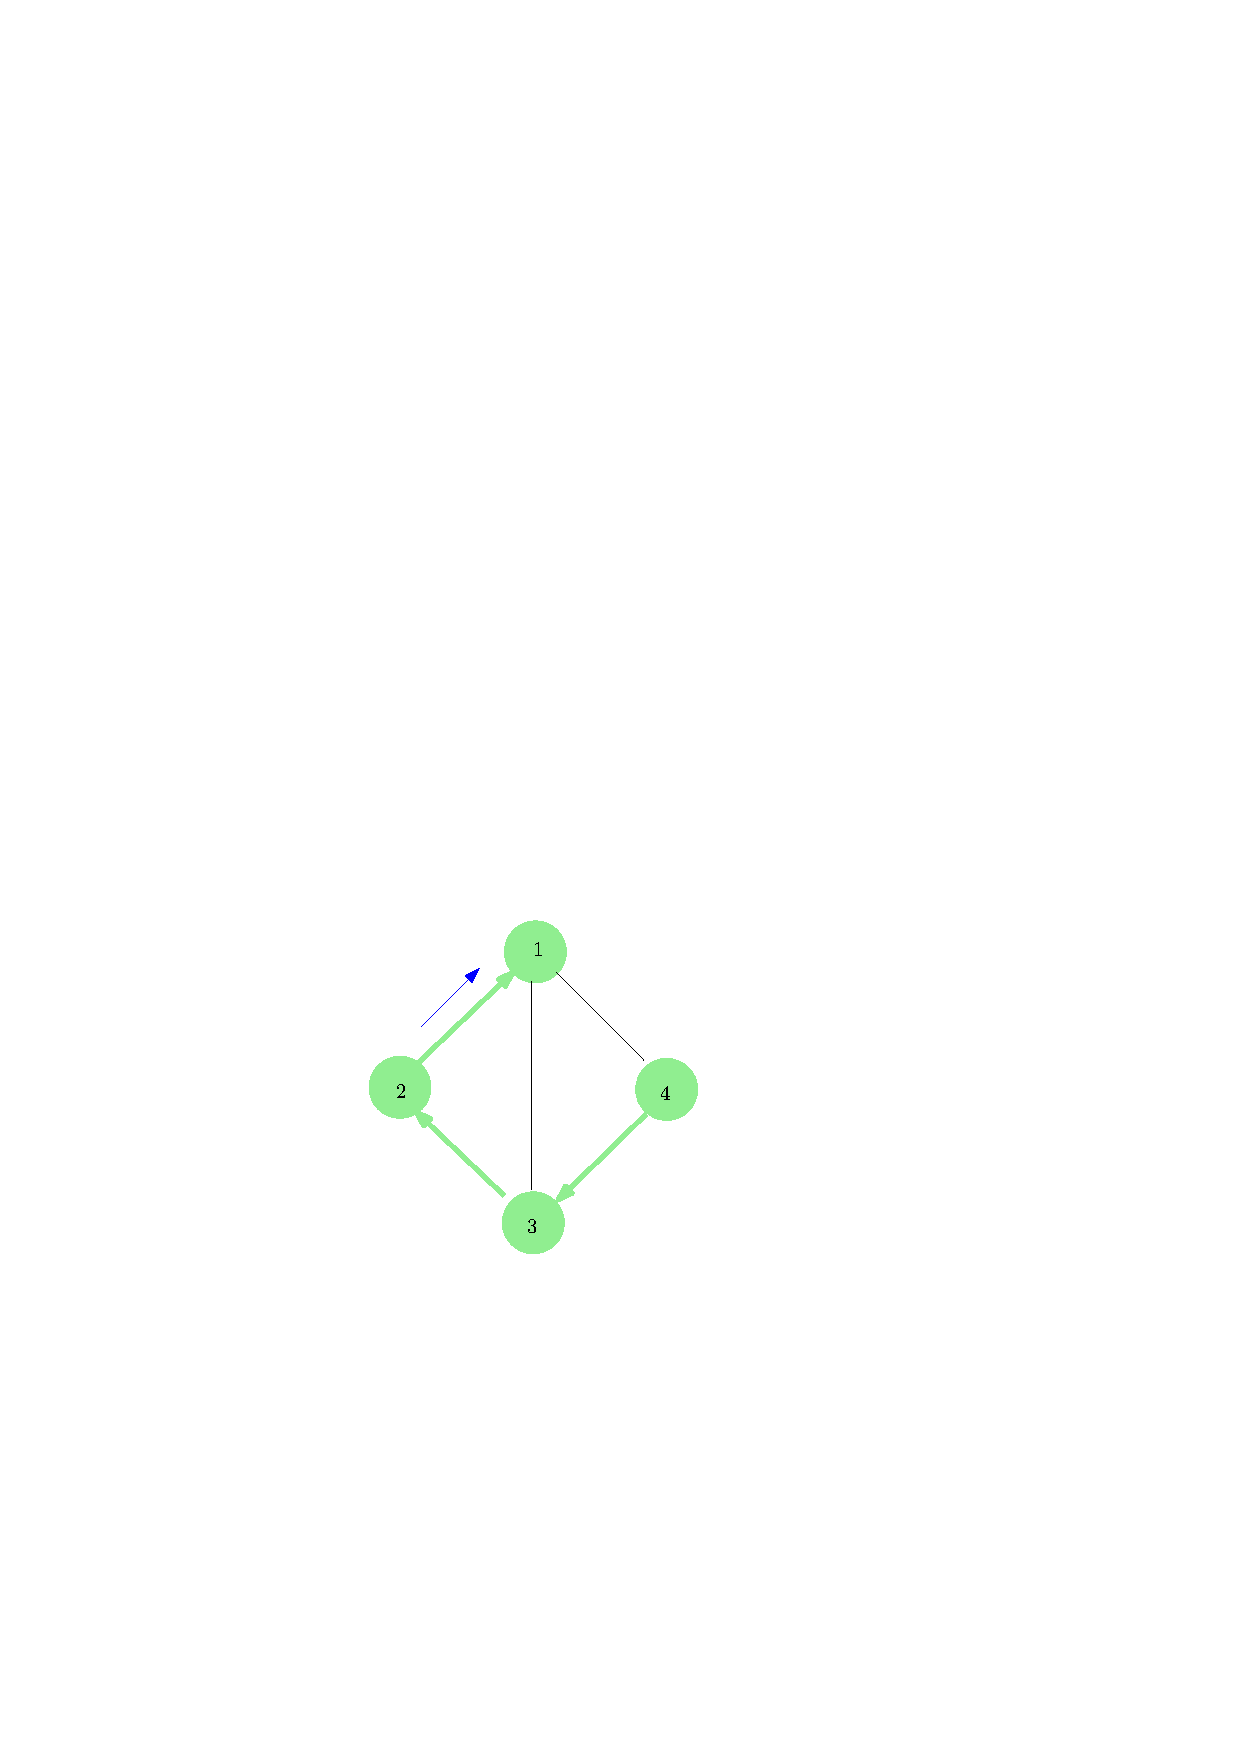
\includegraphics[width=0.32\textwidth]{chapters/background/images/echo/async/notext_f0_8.pdf}}
    \caption[Progression of the asynchronous \textsf{echo} algorithm]{Progression of the asynchronous \textsf{echo} algorithm, starting from round zero before any messages are sent.  Arrows in red mean broadcast messages, while arrows in blue mean convergecast messages.  Despite node 1 being the initiator node, node 4 considers node 3 to be its parent because it first receives a broadcast message from node 3.}
    \label{fig:back:echoasync}
\end{figure}

In the synchronous case, all messages sent out are received simultaneously, and all nodes proceed through their rounds together.  In the asynchronous case, however, messages may arrive at arbitrary times, and nodes proceed through their rounds entirely independently of one another.  The round numbers in the figure mark the point where at least one message has been received by a node.  The nodes react to messages as they arrive, and might do nothing for a time while other nodes are working if no new messages arrive during that time.  Under the asynchronous model, depending on communications topology and speeds, it is possible for the first broadcast message to reach a process to have followed a less direct route from the initiator than might be possible.  Exactly this is seen in \cref{fig:back:echoasync:3}, where node 4 first receives a message from node 3 (and thus marks node 3 as its parent), despite a direct connection to the initiator, node 1.